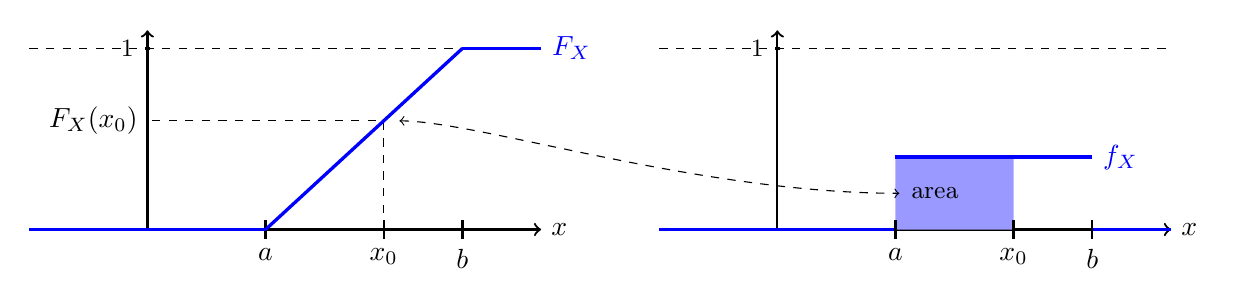
\begin{tikzpicture}[yscale=2.3]
%*** First graph ***
%Axes
\draw[<->, thick] (5,0) node[right] {$x$} --  (0,0) -- (0,1.1);
\draw[thick] (-1.5,0) -- (0,0);

%Ticks
%\foreach \x in {-1,...,4}
%	\draw[xshift = \x cm, thick] (0,-1pt) -- (0,1pt) node[below] {\small $\x$};
\draw[very thick] (1pt,1) -- (-1pt,1) node[left] {\small 1};
\draw[thick] (1.5,.05) -- (1.5,-.05) node[below] {$a$};
\draw[thick] (3,.05) -- (3,-.05) node[below] {$x_0$};
\draw[thick] (4,.05) -- (4,-.05) node[below] {$b$};
\draw[dashed] (3,0)  -- (3,0.6) -- (0,0.6) node[left]{$F_X(x_0)$};

%Dashed horizontal line
\draw[dashed,thin] (-1.5,1) -- (5,1);

%Graph
\draw[very thick,blue] (-1.5,0)--(1.5,0);
\draw[domain=1.5:4, very thick, blue] plot ({\x},{(\x-1.5)/2.5});
	\draw[very thick,blue] (4,1)--(5,1) node[right] {$F_X$};

%*** Second graph ***
\begin{scope}[xshift=8cm]
%Axes
\draw[<->, thick] (5,0) node[right] {$x$} --  (0,0) -- (0,1.1);
\draw[thick] (-1.5,0) -- (0,0);
%\foreach \x in {-1,...,4}
%	\draw[xshift = \x cm, thick] (0,-1pt) -- (0,1pt) node[below] {\small $\x$};

%Area below curve
\fill[blue!40] (1.5,0) -- (1.5,0.4) -- (3,0.4) -- (3,0) -- (1.5,0);

%Dashed horizontal line
\draw[dashed,thin] (-1.5,1) -- (5,1);

%Graph
\draw[very thick,blue] (-1.5,0) -- (1.5,0);
	\draw[very thick,blue] (1.5,0.4) -- (4,0.4) node[right] {$f_X$};
\draw[very thick,blue] (4,0) -- (5,0);

%Ticks
\draw[very thick] (1pt,1) -- (-1pt,1) node[left] {\small 1};
\draw[thick] (1.5,.05) -- (1.5,-.05) node[below] {$a$};
\draw[thick] (3,.05) -- (3,-.05) node[below] {$x_0$};
\draw[thick] (4,.05) -- (4,-.05) node[below] {$b$};

%Area text
\draw (2,0.2) node {\small{area}};
\end{scope}



%Curved long arrow
\draw[<->, dashed, thin] (3.2,0.6) .. controls (4.2,0.6) and (7,0.2) .. (9.55,0.2);
\end{tikzpicture}

